\section{圆的相关题型}

\subsection{点到圆的距离最值}

\begin{theorem}
    这里最常用到的就是 $d_{max} = d + r, d_{min} = d - r$。

    \begin{warning}
        这是和圆距离有关的最值问题中，最常用的式子，请牢记。
    \end{warning}

    \begin{center}
        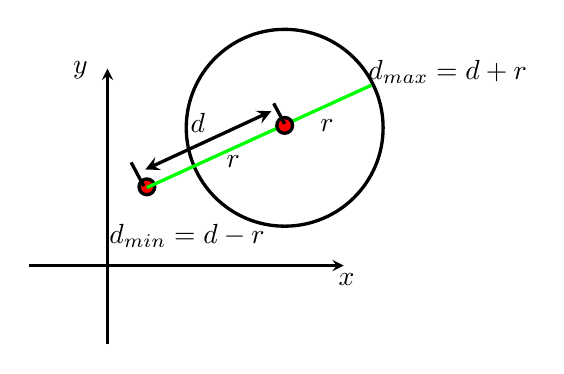
\begin{tikzpicture}
            \node[black, anchor=south west] at (2.81,-1.38) {$x$};
            \node[black, anchor=south west] at (-0.56,1.25) {$y$};
            \draw[draw=black, -stealth, thick, solid] (-1.00,-1.00) -- (3.00,-1.00);
            \draw[draw=black, -stealth, thick, solid] (0.00,-2.00) -- (0.00,1.50);
            \draw[draw=black, very thick, solid] (2.25,0.75) ellipse (1.25 and 1.25);
            \draw[draw=black, fill=red, very thick, solid] (0.50,0.00) circle (0.1);
            \draw[draw=green, very thick, solid] (0.50,-0.01) -- (3.35,1.29);
            \draw[draw=black, fill=red, very thick, solid] (2.25,0.78) circle (0.1);
            \node[black, anchor=south west] at (3.19,1.19) {$d_{max}=d+r$};
            \draw[draw=black, very thick, solid] (0.30,0.31) -- (0.46,0.01);
            \draw[draw=black, very thick, solid] (2.11,1.06) -- (2.25,0.80);
            \draw[draw=black, stealth-stealth, very thick, solid] (0.48,0.22) -- (2.08,0.96);
            \node[black, anchor=south west] at (-0.10,-0.90) {$d_{min}=d-r$};
            \node[black, anchor=south west] at (2.58,0.58) {$r$};
            \node[black, anchor=south west] at (1.39,0.12) {$r$};
            \node[black, anchor=south west] at (0.93,0.56) {$d$};
        \end{tikzpicture}
    \end{center}
\end{theorem}

\begin{example}
    已知 $Q$ 为圆 $C:(x-2)^2+(y-1)^2=1$ 上一动点，$M(7,4)$ ，点 $P$ 为 $x$ 轴上一动点，则 $|P M|+|P Q|$ 的最小值为 $\qquad$
\end{example}

\v{12em}

\subsection{垂径定理}

\begin{theorem}[垂径定理]
    垂直于弦的直径平分这条弦，并且平分弦所对的两条弧。

    \begin{minipage}[c]{0.55\textwidth}
        用几何语言描述为：
        在圆 $O$ 中，若直径 $CD$ 垂直于弦 $AB$ (非直径) 于点 $M$，则：
        \begin{itemize}
            \item 弦被平分：$AM = MB$
            \item 劣弧被平分：$\overset{\frown}{AD} = \overset{\frown}{BD}$
            \item 优弧被平分：$\overset{\frown}{AC} = \overset{\frown}{BC}$
        \end{itemize}

        此定理也说明，直径 $CD$ 是弦 $AB$ 的垂直平分线，具有垂直平分线的性质。
    \end{minipage}
    \begin{minipage}[c]{0.44\textwidth}
        \begin{tikzpicture}[scale=0.7]
            \def\radius{3}
            \coordinate (O) at (0,0);

            \draw (O) circle (\radius);

            \coordinate (A) at (-2.5, -1.65);
            \coordinate (B) at (2.5, -1.65);
            \coordinate (C) at (0, \radius);
            \coordinate (D) at (0, -\radius);
            \coordinate (M) at (0, -1.65);

            \draw (C) -- (D);
            \draw (A) -- (B);
            \draw[dashed] (O) -- (A);
            \draw[dashed] (O) -- (B);

            \fill (O) circle (2pt) node[above right] {$O$};
            \fill (A) circle (2pt) node[below left] {$A$};
            \fill (B) circle (2pt) node[below right] {$B$};
            \fill (C) circle (2pt) node[above] {$C$};
            \fill (D) circle (2pt) node[below] {$D$};
            \fill (M) circle (2pt) node[right=2pt] {$M$};

            \draw ($(M)+(0.2,0)$) -- ($(M)+(0.2,0.2)$) -- ($(M)+(0,0.2)$);
        \end{tikzpicture}
    \end{minipage}

\end{theorem}


\subsection{圆的弦长公式}
\begin{theorem}[弦长公式的应用]
    \begin{minipage}{0.45\textwidth}
        弦长公式是计算圆内任意弦长的重要工具：
        \begin{align*}
            L & = 2\sqrt{r^2-d^2}
        \end{align*}
        其中：
        \begin{itemize}
            \item $L$ 表示弦长
            \item $r$ 是圆的半径
            \item $d$ 是圆心到弦的距离
        \end{itemize}

        由此可知：
        \begin{itemize}
            \item 当 $d=0$ 时，弦长取最大值 $2r$（直径）
            \item 当 $d$ 增大时，弦长减小
            \item 当 $d=r$ 时，弦长为 $0$（圆上一点）
        \end{itemize}
    \end{minipage}
    \begin{minipage}{0.5\textwidth}
        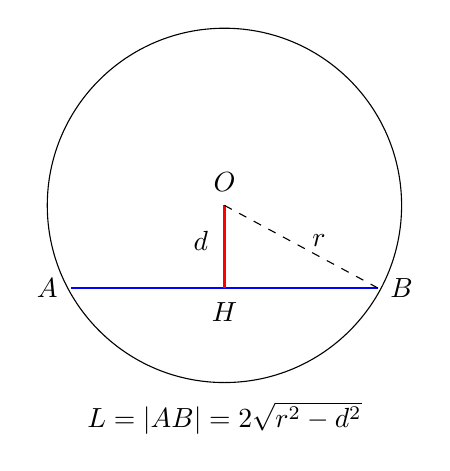
\begin{tikzpicture}[scale=1.5]
            % Draw circle
            \draw (0,0) circle (1.5);

            % Draw chord
            \draw[thick, blue] (-1.3,-0.7) -- (1.3,-0.7);

            % Draw radius and d line
            \draw[thick, red] (0,0) -- (0,-0.7);

            % Draw r line
            \draw[dashed] (0,0) -- (1.3,-0.7);

            % Labels
            \node at (-0.2,-0.3) {$d$};
            \node at (0,0.2) {$O$};
            \node at (0.8,-0.3) {$r$};
            \node at (0,-0.9) {$H$};
            \node at (-1.5,-0.7) {$A$};
            \node at (1.5,-0.7) {$B$};
            \node at (0,-1.8) {$L = |AB| = 2\sqrt{r^2-d^2}$};
        \end{tikzpicture}
    \end{minipage}
\end{theorem}
\begin{example}
    直线 $y=k x+3$ 被圆 $(x-2)^2+(y-3)^2=4$ 截得的弦长为 $2 \sqrt{3}$ ，则直线的倾斜角可能为（ \hspace{2em} ）
    \begin{tasks}(4)
        \task $\frac{5 \pi}{6}$
        \task $\frac{\pi}{3}$
        \task $\frac{2 \pi}{3}$
        \task $\frac{\pi}{6}$
    \end{tasks}
\end{example}

\v{12em}

\begin{example}
    圆 $C$ 过 $(0,3)$、$(4,5)$ 两点，且圆心 $C$ 在直线 $x-y+8=0$ 上．
    \begin{itemize}
        \item[（1）] 求圆 $C$ 的方程；
        \item[（2）] 若直线 $l$ 在 $x$ 轴上的截距是 $y$ 轴上的截距的 2 倍，且被圆 $C$ 截得的弦长为 6 ，求直线 $l$ 的方程。
    \end{itemize}
\end{example}

\v{12em}

\begin{theorem}[弦长的取值范围]
    要分情况讨论：
    \begin{itemize}
        \item 若过一个在圆内的点：$[2\sqrt{R^2-d^2}, 2R]$，此时与圆心的连线垂直。
        \item 若过一个在圆上的点：$[0, 2R]$，直径时是最长的。
    \end{itemize}

    \begin{minipage}{0.5\textwidth}
        \begin{center}
            \begin{tikzpicture}[scale=0.8]
                \draw (0,0) circle (1.5);
                \draw[fill=black] (0,0) circle (1pt) node[below right] {$O$};
                \draw[fill=red] (-0.7,0.5) circle (1.5pt) node[left] {$P$};
                \draw[dashed] (0,0) -- (-0.7,0.5);
                \draw[thick, blue] (-1.54,-0.59) -- (0.14,1.59);
                \node at (-1.4,-0.8) {$L_{min}$};
                \draw[thick, red] (-1.5,1.07) -- (1.5,-1.07);
                \node at (0.7,-1.0) {$L_{max}$};
                \node at (0,-2) {过圆内点的弦长范围};
            \end{tikzpicture}
        \end{center}
    \end{minipage} %
    \begin{minipage}{0.5\textwidth}
        \begin{center}
            \begin{tikzpicture}[scale=0.8]
                % Draw circle
                \draw (0,0) circle (1.5);
                \draw[fill=black] (0,0) circle (1pt) node[below right] {$O$};

                % Point on circle
                \draw[fill=red] (1.5,0) circle (1.5pt) node[right] {$P$};

                % Max chord case - diameter
                \draw[thick, blue] (-1.5,0) -- (1.5,0);
                \node at (0,0.5) {$L_{max}=2r$};

                % Min chord case - tangent at P
                \draw[thick, red] (1.5,-0.1) -- (1.5,0.1);
                \node at (2,-1) {$L_{min}=0$};

                \node at (0,-2) {过圆上点的弦长范围};
            \end{tikzpicture}
        \end{center}
    \end{minipage}
\end{theorem}

\begin{example}
    直线 $m x-y+1-m=0$ 与圆 $x^2+y^2=4$ 相交，则弦长可能为（ \hspace{2em} ）
    \begin{tasks}(4)
        \task $2$
        \task $3$
        \task $\sqrt{10}$
        \task $5$
    \end{tasks}
\end{example}

\v{10em}

\subsection{圆和斜率构造}

\begin{theorem}[求直线与圆相切]
    当直线与圆相切时，圆心到直线的距离等于圆的半径。这是判断直线与圆相切的充要条件。
    \begin{center}
        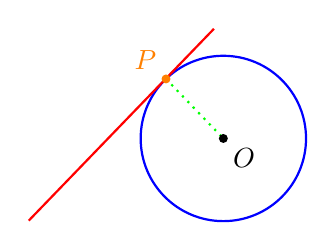
\begin{tikzpicture}[scale=0.7]
            % Draw circle
            \draw[draw=blue, thick, solid] (0.50,0.50) ellipse (1.50 and 1.50);
            % Draw tangent line
            \draw[draw=red, thick, solid] (-3.03,-0.99) -- (0.33,2.49);
            % Draw radius to point of tangency
            \draw[draw=green, thick, dotted] (-0.54,1.58) -- (0.50,0.50);
            % Add circle center
            \filldraw[black] (0.50,0.50) circle (2pt) node[below right] {$O$};
            % Add point of tangency
            \filldraw[orange] (-0.54,1.58) circle (2pt) node[above left] {$P$};
        \end{tikzpicture}
    \end{center}
\end{theorem}

\begin{example}
    已知实数 $x, y$ 满足 $x^2+y^2-4 x-2 y-4=0$ ，则 $\frac{y-1}{x+3}$ 的最大值是 （\qquad）
    \begin{tasks}(4)
        \task $\frac{1}{2}$
        \task $\frac{\sqrt{2}}{2}$
        \task $\frac{3}{4}$
        \task 1
    \end{tasks}
\end{example}

\v{12em}

\begin{example}
    已知圆 $C: x^2+y^2-4x+6y+4=0$ 与直线 $l: 3x-4y+m=0$ 相切，求参数 $m$ 的值。
\end{example}

\v{12em}

\subsection{两点间的距离构造}

\begin{theorem}
    两点间的距离为 $d=\sqrt{(x_2-x_1)^2+(y_2-y_1)^2}$。

    类似 $(x-1)^2+y^2$ 的式子都可以构造为两点间的距离。
\end{theorem}

\begin{example}
    已知圆 $x^2+(y-2)^2=4$ 上一点 $P(m, n)$ ，则 $\sqrt{m^2+n^2}$ 的最大值为 \underline{\qquad}
\end{example}

\v{12em}

\begin{example}
    实数 $x$、$y$ 满足 $x^2+y^2=4$ ，则 $(x-4)^2+(y+3)^2$ 的最大值是 \underline{\qquad}
\end{example}

\v{12em}

\begin{example}
    已知实数 $x, y$ 满足方程 $x=\sqrt{1-y^2}$ ，则（ \qquad）
    \begin{itemize}
        \item $(x-2)^2+y^2$ 的取值范围是 $[1, \sqrt{5}]$
        \item $\frac{y+2}{x+1}$ 的取值范围是 $\left[\frac{3}{4}, 3\right]$
    \end{itemize}
\end{example}

\v{12em}


\subsection{轴对称与将军饮马}

\begin{theorem}[轴对称与点到圆的距离]
    将军饮马需要让其中一个点作对称点。

    \begin{center}
        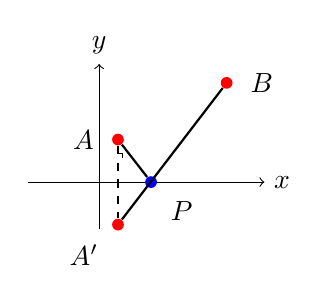
\begin{tikzpicture}[scale=0.6]
            % Coordinate axes
            \draw[->] (-1.5,-1.5) -- (3.5,-1.5) node[right] {$x$};
            \draw[->] (0,-2.5) -- (0,1) node[above] {$y$};

            % Points
            \node[circle, fill=blue, inner sep=1.5pt, label={[label distance=0.1cm]below right:$P$}] (P) at (1.1,-1.5) {};
            \node[circle, fill=red, inner sep=1.5pt, label={[label distance=0.1cm]left:$A$}] (A) at (0.4,-0.6) {};
            \node[circle, fill=red, inner sep=1.5pt, label={[label distance=0.1cm]right:$B$}] (B) at (2.7,0.6) {};

            % Reflection point A'
            \node[circle, fill=red, inner sep=1.5pt, label={[label distance=0.1cm]below left:$A'$}] (Aprime) at (0.4,-2.4) {};

            % Lines
            \draw[thick] (Aprime) -- (B);
            \draw[thick, dashed] (A) -- (Aprime);

            % Right angle symbol
            \draw (0.4,-0.9) -- (0.5,-0.9) -- (0.5,-1.0);

            % Additional line (optional)
            \draw[thick] (A) -- (P);
        \end{tikzpicture}
    \end{center}
\end{theorem}

\begin{example}
    已知圆 $M_1:(x-2)^2+(y-1)^2=2$ ，圆 $M_2: x^2+y^2-2 x+2 y+1=0$ ，点 $P$ 为 $y$ 轴上的动点，则 $|P M_1|+|P M_2|$ 的最小值为（ \hspace{2em} ）
    \begin{tasks}(4)
        \task $3$
        \task $\sqrt{13}$
        \task $\sqrt{10}$
        \task $\sqrt{5}$
    \end{tasks}
\end{example}

\v{12em}

\begin{theorem}[圆距离的转换]
    先使用点到圆的距离的不等式进行第一步转换，再进行将军饮马：

    假设 K 是定点，N 是圆上的一个动点，有：
    $$
        |KN| \geq |KO| - r, \quad |KN| \leq |KO| + r
    $$
\end{theorem}

\begin{example}
    在平面直角坐标系中，军营所在区域的边界为 $x^2+y^2=1$ ，河岸所在直线方程为 $x+y=3$ ，将军从点 $A(0,2)$ 处出发，先到河边饮马，然后再返回军营，如果将军只要到达军营所在区域即回到军营，则这个将军所经过的最短路程为（ \hspace{2em} ）
    \begin{tasks}(4)
        \task $\sqrt{5}$
        \task $\sqrt{5}-1$
        \task $\sqrt{10}$
        \task $\sqrt{10}-1$
    \end{tasks}
\end{example}

\v{12em}

\begin{example}
    已知圆 $C:(x+2)^2+(y-1)^2=8$ ，直线 $l: 4 x-y-8=0, ~ M$ 为直线 $l$ 上一动点，$N$ 为圆 $C$ 上一动点，定点 $P(2,3)$ ，则 $|M N|+|M P|$ 的最小值为 （\qquad）

    \begin{center}
        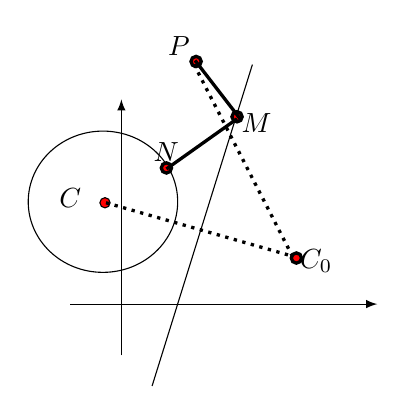
\begin{tikzpicture}[scale = 1.3]
            \draw[draw=black, -latex, thin, solid] (-2.00,0.00) -- (1.00,0.00);
            \draw[draw=black, -latex, thin, solid] (-1.50,-0.50) -- (-1.50,2.00);
            \draw[draw=black, thin, solid] (-1.68,1.00) ellipse (0.73 and 0.69);
            \draw[draw=black, fill=red, thin, solid] (-1.66,0.99) circle (0.05);
            \draw[draw=black, thin, solid] (-0.22,2.34) -- (-1.20,-0.80);
            \draw[draw=black, very thick, dotted] (-1.65,0.99) -- (0.20,0.46);
            \draw[draw=black, fill=red, very thick, solid] (0.21,0.45) circle (0.05);
            \draw[draw=black, fill=red, very thick, solid] (-0.37,1.83) circle (0.05);
            \draw[draw=black, fill=red, very thick, solid] (-1.06,1.33) circle (0.05);
            \node[black, anchor=south west] at (-1.28,1.30) {$N$};
            \node[black, anchor=south west] at (-0.42,1.58) {$M$};
            \node[black, anchor=south west] at (-2.20,0.85) {$C$};
            \node[black, anchor=south west] at (0.15,0.21) {$C_0$};
            \draw[draw=black, very thick, solid] (-0.37,1.81) -- (-1.06,1.32);
            \draw[draw=black, fill=red, very thick, solid] (-0.77,2.37) circle (0.05);
            \node[black, anchor=south west] at (-1.14,2.33) {$P$};
            \draw[draw=black, very thick, solid] (-0.34,1.81) -- (-0.78,2.38);
            \draw[draw=black, very thick, dotted] (-0.79,2.34) -- (0.18,0.45);
        \end{tikzpicture}
    \end{center}

    \begin{tasks}(4)
        \task $\sqrt{2}$
        \task $\sqrt{3}$
        \task $2 \sqrt{2}$
        \task $2 \sqrt{3}$
    \end{tasks}
\end{example}

\v{2em}

\begin{example}
    已知圆 $C:(x-1)^2+(y-2)^2=1$ ，点 $A(7,6), ~ B$ 为圆 $C$ 上的动点，$Q$ 为 $x$ 轴上的动点，则 $\{|Q A|+|Q B|\}_{min}$ = \underline{\qquad}
\end{example}

\vspace{10em}

\pagebreak

\subsection{圆和圆的位置关系}

\begin{theorem}[圆与圆的位置关系]
    通过比较两圆的圆心距 $d$ 与两圆半径之和 $R+r$、半径之差 $|R-r|$ 的大小，可以判断两圆的位置关系。

    \begin{center}
        \begin{tabular}{|c|c|c|}
            \hline
            位置关系 & 圆心距 $d$ 与半径关系         & 图示特征              \\
            \hline
            外离   & $d > R + r$           & 两圆完全分离            \\
            \hline
            外切   & $d = R + r$           & 两圆只有一个公共点         \\
            \hline
            相交   & $|R - r| < d < R + r$ & 两圆有两个交点           \\
            \hline
            内切   & $d = |R - r|$         & 两圆只有一个公共点，一圆在另一圆内 \\
            \hline
            内含   & $d < |R - r|$         & 一个圆完全包含在另一个圆内     \\
            \hline
        \end{tabular}
    \end{center}

    % 上排：外离、外切、相交
    \begin{center}
        \begin{tikzpicture}[scale=0.6]
            % Case 1: Circles are completely separate (d > R + r)
            \draw (-2.5,0) circle (1);
            \draw (0.5,0) circle (1.5);
            \draw[dashed] (-2.5,0) -- (0.5,0);
            \node at (-1,0.3) {$d$};
            \node at (-2.5,0) {$\bullet$};
            \node at (0.5,0) {$\bullet$};
            \node at (-1,-1.5) {外离 ($d > R + r$)};

            % Case 2: Circles touch at one point (d = R + r)
            \draw (5,0) circle (1);
            \draw (7.5,0) circle (1.5);
            \draw[dashed] (5,0) -- (7.5,0);
            \node at (6.25,0.3) {$d$};
            \node at (5,0) {$\bullet$};
            \node at (7.5,0) {$\bullet$};
            \node at (6.25,-1.5) {外切 ($d = R + r$)};

            % Case 3: Circles intersect at two points (|R - r| < d < R + r)
            \draw (12,0) circle (1.5);
            \draw (14,0) circle (1.7);
            \draw[dashed] (12,0) -- (14,0);
            \node at (13,0.3) {$d$};
            \node at (12,0) {$\bullet$};
            \node at (14,0) {$\bullet$};
            \node at (13,-1.5) {相交 ($|R-r| < d < R+r$)};
        \end{tikzpicture}
    \end{center}

    % 下排：内切、内含
    \begin{center}
        \begin{tikzpicture}[scale=0.6]
            % Case 4: One circle inside another, touching at one point (d = |R - r|)
            \draw (0,0) circle (2);
            \draw (1.5,0) circle (0.5);
            \draw[dashed] (0,0) -- (1.5,0);
            \node at (0.75,0.3) {$d$};
            \node at (0,0) {$\bullet$};
            \node at (1.5,0) {$\bullet$};
            \node at (0.75,-1.5) {内切 ($d = |R - r|$)};

            % Case 5: One circle completely inside another (d < |R - r|)
            \draw (5,0) circle (2);
            \draw (5.8,0) circle (0.7);
            \draw[dashed] (5,0) -- (5.8,0);
            \node at (5.4,0.3) {$d$};
            \node at (5,0) {$\bullet$};
            \node at (5.8,0) {$\bullet$};
            \node at (5.4,-1.5) {内含 ($d < |R - r|$)};
        \end{tikzpicture}
    \end{center}
\end{theorem}

\begin{example}
    设圆 $C_1: x^2+y^2=4$ ，圆 $C_2: x^2+y^2-6 x+8=0$ ，则圆 $C_1, ~ C_2$ 的位置关系是（ \hspace{2em} ）
    \begin{tasks}(4)
        \task 内切
        \task 外切
        \task 相交
        \task 相离
    \end{tasks}
\end{example}

\v{6em}

\begin{example}
    圆 $C_1:(\mathrm{x}+1)^2+(\mathrm{y}-3)^2=36$ 与圆 $C_2:(x-2)^2+(y+1)^2=1$的位置关系是 （\qquad）
    \begin{tasks}(4)
        \task 相交
        \task 内切
        \task 外切
        \task 外离
    \end{tasks}
\end{example}

\v{6em}

\begin{example}
    ＂$a^2+b^2<R^2$＂是＂圆 $(x-a)^2+(y-b)^2=R^2$ 与坐标轴有四个交点＂的 （\qquad）条件
\end{example}

\v{8em}

\begin{example}
    已知圆 $C_1:(x-2 m)^2+(y-2 m)^2=9(m-2)$ 与圆 $C_2: x^2+y^2-8 x-8 y+34-m=0$

    则＂$m=4$＂是＂圆 $C_1$ 与圆 $C_2$ 外切＂的 （\qquad）条件
\end{example}

\v{8em}

\subsection{两圆公共弦问题}

\begin{theorem}[两圆公共弦问题]
    两圆方程作差即可得到它们的公共弦所在直线的方程。然后利用圆心到公共弦的距离、半径和半弦长构成的直角三角形，通过勾股定理求出弦长。
\end{theorem}
\begin{example}
    若圆 $x^2+y^2+2 x-4 y-5=0$ 与 $x^2+y^2+2 x-1=0$ 相交于 $A$、$B$ 两点，则公共弦 $A B$ 的长是（ \hspace{2em} ）。
    \begin{tasks}(4)
        \task $1$
        \task $2$
        \task $3$
        \task $4$
    \end{tasks}
\end{example}

\v{10em}

\begin{example}
    圆 $C_1: x^2+y^2+2 x-8 y-8=0$ 与圆 $C_2: x^2+y^2+4 x-4 y-4=0$ 的公共弦长为（ \hspace{2em} ）
    \begin{tasks}(4)
        \task $\frac{\sqrt{55}}{5}$
        \task $\frac{2 \sqrt{55}}{5}$
        \task $\frac{3 \sqrt{55}}{5}$
        \task $\frac{4 \sqrt{55}}{5}$
    \end{tasks}
\end{example}

\v{10em}

\subsection{圆的切线方程}

\begin{theorem}[过圆外一点的切线方程]
    圆心到动直线的距离等于半径。

    \begin{center}
        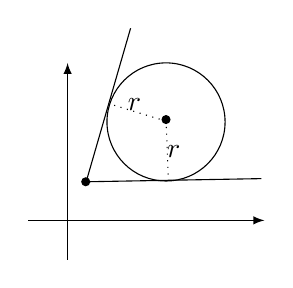
\begin{tikzpicture}
            \draw[draw=black, -latex, thin, solid] (-2.00,0.00) -- (1.00,0.00);
            \draw[draw=black, -latex, thin, solid] (-1.50,-0.50) -- (-1.50,2.00);
            \draw[draw=black, thin, solid] (-0.25,1.25) ellipse (0.75 and 0.75);
            \draw[draw=black, fill=black, thin, solid] (-1.27,0.49) circle (0.05);
            \draw[draw=black, thin, solid] (-1.27,0.47) -- (-0.70,2.44);
            \draw[draw=black, thin, solid] (-1.26,0.49) -- (0.96,0.53);
            \draw[draw=black, fill=black, thin, solid] (-0.25,1.28) circle (0.05);
            \draw[draw=black, thin, dotted] (-0.25,1.26) -- (-0.97,1.48);
            \draw[draw=black, thin, dotted] (-0.25,1.27) -- (-0.22,0.52);
            \node[black, anchor=south west] at (-0.86,1.27) {$r$};
            \node[black, anchor=south west] at (-0.36,0.67) {$r$};
        \end{tikzpicture}
    \end{center}
\end{theorem}

\begin{example}
    已知圆 $C: x^2+y^2-4x+6y+4=0$ 与直线 $l: 3x-4y+m=0$ 相切，求参数 $m$ 的值。
\end{example}

\v{10em}

\begin{example}
    过点 $(-1,0)$ 作直线 $l$ 与圆 $(x-2)^2+(y-1)^2=1$ 相切，斜率的最大值为 $M$ ，若 $a+b=M, ~ a>0, ~ b>0$ ，则 $\frac{1}{a}+\frac{4}{b}$ 的最小值是 （\qquad）
    \begin{tasks}(4)
        \task 12
        \task 9
        \task $\frac{27}{4}$
        \task $\frac{28}{3}$
    \end{tasks}
\end{example}

\vspace{10em}

\begin{example}
    已知圆 $C: x^2+y^2-6 x-8 y+21=0$ ，直线 $l$ 过点 $A(1,0)$ ．
    \begin{enumerate}
        \item 若直线 $l$ 与圆 $C$ 相切，求直线 $l$ 的方程；

        \item 当直线 $l$ 的斜率存在且与圆 $C$ 相切于点 $B$ 时，求 $|A B|$ ．
    \end{enumerate}
\end{example}

\v{10em}

\begin{theorem}[过圆上一点的切线方程]
    若已知点 $P(x_0, y_0)$ 在圆 $(x-a)^2+(y-b)^2=r^2$ 上，则过该点的切线方程为 $(x_0-a)(x-a)+(y_0-b)(y-b)=r^2$。
\end{theorem}

\begin{example}
    已知圆 $C:(x-4)^2+(y+5)^2=2$ ，则圆 $C$ 在点 $P(3,-4)$ 处的切线方程为 \underline{\qquad}
\end{example}

\begin{tips}
    当然，可以直接使用切线的垂直性质，求出斜率。
\end{tips}

\v{10em}

\subsection{两圆公切线条数}

\begin{theorem}[两圆公切线条数]
    两圆有且仅有三条公切线是两圆外切的充要条件。因此，两圆的圆心距等于两圆半径之和。
    \begin{enumerate}
        \item 四条公切线：相离
        \item 三条公切线：外切
        \item 两条公切线：相交
        \item 一条公切线：内切
    \end{enumerate}
\end{theorem}

\begin{example}
    已知两圆 $C_1: x^2+y^2=1, C_2:(x-1)^2+(y-1)^2=r^2(r>1)$ ，若两圆有且仅有两条公切线，则 $r$ 的取值范围为
\end{example}

\begin{solution}
    相交：
    $$
        \begin{aligned}
            \quad & R_1-R_2<C_1 C_2<R_1+R_2              \\
                  & r-1<\sqrt{1^2+1^2}<r+1               \\
                  & \therefore \left\{\begin{array}{l}
                                          r-1<\sqrt{2} \\
                                          \sqrt{2}<r+1
                                      \end{array}\right.
        \end{aligned}
    $$
\end{solution}

\begin{example}
    若圆 $C_1: x^2+y^2-2 a y=0(a>0)$ 与圆 $C_2: x^2+y^2-4 x+3=0$ 有且仅有三条公切线，则 $a$ 的值为 \underline{\qquad}.
\end{example}

\v{8em}

\begin{example}
    已知圆 $C_1:(x-2)^2+(y+4)^2=16$ ，圆 $C_2: x^2+y^2+2 x-3=0$ ，则两圆的公切线的条数为 （\qquad）
    \begin{tasks}(4)
        \task 1
        \task 2
        \task 3
        \task 4
    \end{tasks}
\end{example}

\v{8em}

\begin{example}
    已知两圆 $x^2+y^2=1, (x-1)^2+(y-1)^2=r^2(r>1)$ ，若两圆有且仅有两条公切线，则 $r$ 的取值范围为 \underline{\qquad}.
\end{example}

\v{8em}

\subsection{圆的参数方程及其应用}

\begin{theorem}[圆的参数方程]
    圆 $C: (x-a)^2+(y-b)^2=r^2$ 的参数方程可表示为：
    $$
        \begin{cases}
            x = a + r\cos\theta \\
            y = b + r\sin\theta
        \end{cases}
    $$
    其中 $\theta \in [0, 2\pi)$ 是参数。通过这种表示，圆上任意一点的坐标都可以用参数 $\theta$ 表示，便于求解圆上点满足特定条件的问题。
\end{theorem}

\begin{example}
    已知圆 $C: x^2+y^2=4$ 上的点 $P(x,y)$ 满足 $\overrightarrow{OP} \cdot \overrightarrow{OA} = 2\sqrt{2}$，其中 $O$ 是坐标原点，$A(2,0)$。
    \begin{itemize}
        \item[(1)] 求点 $P$ 的坐标；
        \item[(2)] 设 $Q$ 是圆 $C$ 上的另一点，若 $\overrightarrow{PQ} \perp \overrightarrow{OA}$，求线段 $PQ$ 的长度。
    \end{itemize}
\end{example}

\v{12em}

\begin{example}
    若点 $P(x, y)$ 在圆 $(x-3)^2+(y-\sqrt{3})^2=6$ 上运动，求：
    \begin{enumerate}
        \item $\frac{y}{x}$ 的最大值；
        \item $x+y$ 的最值．
    \end{enumerate}
\end{example}

\v{12em}

\begin{theorem}[圆的切线长度]
    设点 $P$ 到圆心 $O$ 的距离为 $d$，圆的半径为 $r$，则过点 $P$ 的切线长度为 $L = \sqrt{d^2 - r^2}$（当 $d > r$ 时）。
\end{theorem}

\begin{example}
    已知动点 $M, N$ 分别在圆 $C_1:(x-1)^2+(y-2)^2=1$ 和 $C_2:(x-3)^2+(y-4)^2=3$ 上，动点 $P$ 在 $x$ 轴上，则（ \hspace{2em} ）
    \begin{tasks}(2)
        \task  圆 $C_2$ 的半径为 3
        \task  圆 $C_1$ 和圆 $C_2$ 相离
        \task  $|P M|+|P N|$ 的最小值为 $2 \sqrt{10}$
        \task  过点 $P$ 做圆 $C_1$ 的切线，则切线长最短为 $\sqrt{3}$
    \end{tasks}
\end{example}

\v{12em}

\subsection*{练习题}

\begin{example}
    已知 $C: x^2+y^2-6 x=0$ ，则下述正确的是（ \hspace{2em} ）
    \begin{tasks}(2)
        \task 圆 $C$ 的半径 $r=3$
        \task 点 $(1,2 \sqrt{2})$ 在圆 $C$ 的内部
        \task* 圆 $C$ 与圆 $x^2+y^2+2 x+4 y-6=0$ 的公共弦所在直线方程为 $4 x+2 y-3=0$
        \task 圆 $C':(x+1)^2+y^2=4$ 与圆 $C$ 相交
    \end{tasks}
\end{example}

\v{12em}

% \subsection{解答题}
% \begin{theorem}[直线系与参数范围]
%     \begin{itemize}
%         \item[（1）] 将直线方程整理为关于参数 $a$ 的形式 $a(2x-y) + (-3x+y+1) = 0$，令系数同时为零，解方程组即可求得定点坐标。
%         \item[（2）] 直线不经过第二象限，意味着其斜率 $k \ge 0$ 且其 $y$ 轴截距 $b \le 0$（或斜率不存在时，$x$ 截距大于等于0）。通过分析斜率和截距与 $a$ 的关系来求解 $a$ 的范围。
%         \item[（3）] 写出两截距关于参数 $a$ 的表达式，进而写出面积的表达式，利用基本不等式求其最小值。
%     \end{itemize}
% \end{theorem}
% \begin{example}
%     已知直线 $l:(a-1) y=(2 a-3) x+1$ ．
%     \begin{itemize}
%         \item[（1）] 求证：直线 $l$ 过定点；
%         \item[（2）] 若直线 $l$ 不经过第二象限，求实数 $a$ 的取值范围；
%         \item[（3）] 若直线 $l$ 与两坐标轴的正半轴围成的三角形面积最小，求 $l$ 的方程．
%     \end{itemize}
% \end{example}

% \v{12em}

% \subsection{解答题}
% \begin{theorem}[直线系与最值问题]
%     \begin{itemize}
%         \item[（1）] 将方程整理为 $a(x-2) + (x+y-5)=0$ 的形式，解方程组 $\begin{cases} x-2=0 \\ x+y-5=0 \end{cases}$ 即可找到定点。
%         \item[（2）] 用参数 $a$ 表示出两截距，进而表示出三角形面积 $S$。利用换元法和基本不等式求 $S$ 的最小值。
%         \item[（3）] 将两截距的表达式设为正整数，通过分析表达式的结构和 $a$ 为正整数的条件，求解不定方程。
%     \end{itemize}
% \end{theorem}
% \begin{example}
%     设直线 $l$ 的方程为 $(a+1) x+y-5-2 a=0(a \in \mathrm{R})$ ．
%     \begin{itemize}
%         \item[（1）] 求证：不论 $a$ 为何值，直线必过一定点 $P$ ；
%         \item[（2）] 若直线 $l$ 分别与 $x$ 轴正半轴，$y$ 轴正半轴交于点 $A\left(x_A, 0\right), B\left(0, y_B\right)$ ，当 $\Delta A O B$ 面积最小时，求此时的直线方程；
%         \item[（3）] 当直线 $l$ 在两坐标轴上的截距均为正整数且 $a$ 也为正整数时，求直线 $l$ 的方程．
%     \end{itemize}
% \end{example}

% \v{12em}

% % =============================================
% % 第三批题目 (来自图片)
% % =============================================

% \subsection{解答题}
% \begin{theorem}[线段垂直平分线与点到直线距离]
%     \begin{itemize}
%         \item[(1)] 线段的垂直平分线满足两个条件：过线段中点，且与线段所在直线垂直。
%         \item[(2)] 一条直线与两相异定点 $A, B$ 的距离相等，意味着该直线或者平行于直线 $AB$，或者经过线段 $AB$ 的中点。
%     \end{itemize}
% \end{theorem}
% \begin{example}
%     已知点 $A(1,3), B(5,7)$．
%     \begin{itemize}
%         \item[(1)] 求线段 $AB$ 垂直平分线所在直线的方程；
%         \item[(2)] 若直线 $l$ 过 $(-1,0)$，且点 $A$、$B$ 到直线 $l$ 的距离相等，求直线 $l$ 的方程．
%     \end{itemize}
% \end{example}

% \v{12em}

% \subsection{解答题}
% \begin{theorem}[直线系与圆的综合应用]
%     \begin{itemize}
%         \item[(1)] 首先将含参的直线方程整理为 $m(x+2y-5) + (-x+3) = 0$ 的形式，求出其恒过的定点。然后判断该定点与圆的位置关系，若定点在圆内，则直线与圆恒相交。
%         \item[(2)] 过圆内一定点的所有弦中，最短的弦是与过该定点的直径垂直的弦。此时，圆心到弦的距离最大，等于圆心与该定点之间的距离。利用弦长公式 $L=2\sqrt{r^2-d^2}$ 即可求出最短弦长。
%     \end{itemize}
% \end{theorem}
% \begin{example}
%     已知直线 $l: (m-1)x + 2my - 5m + 3 = 0, m \in \mathrm{R}$ 和圆 $C: (x-2)^2 + (y-1)^2 = 4$．
%     \begin{itemize}
%         \item[(1)] 证明：圆 $C$ 与直线 $l$ 恒相交；
%         \item[(2)] 求直线 $l$ 被圆 $C$ 截得的弦长的最小值．
%     \end{itemize}
% \end{example}

% \v{12em}

% \subsection{选择题}
% \begin{theorem}[抛物线定义与圆的切线长]
%     利用圆的切线长公式 $l^2 = |PC|^2 - r^2$ 建立方程，其中 $P$ 为切点，$C$ 为圆心。将点 $P$ 的坐标代入，并结合点 $P$ 在抛物线上满足的方程 $y^2=2px$，解出点 $P$ 的横坐标。最后根据抛物线的定义，点 $P$ 到准线的距离等于 $x_P + p/2$。
% \end{theorem}

% \begin{example}
%     已知点 $P$ 在抛物线 $M: y^2=8 x$ 上，过点 $P$ 作圆 $C:(x-4)^2+y^2=1$ 的切线，若切线长为 $2 \sqrt{6}$ ，则点 $P$ 到 $M$ 的准线的距离为（\quad）
%     \begin{tasks}(4)
%         \task $5$
%         \task $6$
%         \task $7$
%         \task $4 \sqrt{2}$
%     \end{tasks}
% \end{example}

% \v{12em}

% \subsection{选择题}
% \begin{theorem}[圆的切线性质与向量点积]
%     由圆的切线性质可知，$PM \perp MC$，其中 $C$ 为圆心，$M$ 为切点。因此 $\解三角形 PMC$ 是直角三角形。利用向量点积的几何意义，$\overrightarrow{PM} \cdot \overrightarrow{PC} = |\overrightarrow{PM}||\overrightarrow{PC}|\cos\angle MPC = |\overrightarrow{PM}|^2$。问题转化为求 $|PM|^2$ 的最小值。根据切线长公式 $|PM|^2=|PC|^2-r^2$，求 $|PM|$ 的最小值等价于求动点 $P$ 到圆心 $C$ 的距离 $|PC|$ 的最小值。
% \end{theorem}

% \begin{example}
%     在平面直角坐标系 $x O y$ 中，已知圆 $C:(x-1)^2+y^2=4, ~ P$ 为直线 $l: x+y+3=0$ 上的一个动点，过点 $P$ 作圆 $C$ 的切线 $P M$ ，切点为点 $M$ ，当 $|P M|$ 最小时，则 $\overrightarrow{P M} \cdot \overrightarrow{P C}$ 的值为（\quad）
%     \begin{tasks}(4)
%         \task $4$
%         \task $\sqrt{2}$
%         \task $2$
%         \task $3$
%     \end{tasks}
% \end{example}

% \v{12em}

% \subsection{多选题}
% \begin{theorem}[圆与圆的位置关系及最值问题]
%     A. 由圆的标准方程 $(x-a)^2+(y-b)^2=r^2$ 直接读出半径。B. 比较圆心距与两半径之和、差判断位置关系。C. $|PM|+|PN|$ 的最小值模型，通常利用轴对称转化为两定点间距离问题，再减去相应半径。D. 过点 $P$ 的切线长公式为 $l^2 = |PC|^2 - r^2$，其最小值取决于 $|PC|$ 的最小值。
% \end{theorem}
% \begin{example}
%     已知动点 $M, N$ 分别在圆 $C_1:(x-1)^2+(y-2)^2=1$ 和 $C_2:(x-3)^2+(y-4)^2=3$ 上，动点 $P$ 在 $x$ 轴上，则（\quad）
%     \begin{itemize}
%         \item 圆 $C_2$ 的半径为 3
%         \item 圆 $C_1$ 和圆 $C_2$ 相离
%         \item $|P M|+|P N|$ 的最小值为 $2 \sqrt{10}$
%         \item 过点 $P$ 做圆 $C_1$ 的切线，则切线长最短为 $\sqrt{3}$
%     \end{itemize}
% \end{example}

% \v{12em}

% \subsection{多选题}
% \begin{theorem}[直线系与圆的综合应用]
%     A. 将直线方程整理为关于参数 $m$ 的形式，解出与 $m$ 无关的定点坐标。B. 令 $x=0$ 求圆与 $y$ 轴的交点，计算弦长。C. 判断定点与圆的位置关系，若定点在圆内，则直线与圆恒相交。D. 过圆内定点的最短弦为与定点和圆心连线垂直的弦。
% \end{theorem}
% \begin{example}
%     已知圆 $C:(x-1)^2+(y-2)^2=25$ ，直线 $l:(2 m+1) x+(m+1) y-7 m-4=0$ ．则下列命题正确的有（\quad）
%     \begin{itemize}
%         \item 直线 $l$ 恒过定点 $(3,1)$
%         \item 圆 $C$ 被 $y$ 轴截得的弦长为 $2 \sqrt{6}$
%         \item 直线 $l$ 与圆 $C$ 恒相交
%         \item 直线 $l$ 被圆 $C$ 截得弦长最短时，直线 $l$ 的方程为 $2 x-y-5=0$
%     \end{itemize}
% \end{example}

% \v{12em}

% \subsection{填空题}
% \begin{theorem}[点到圆的距离与几何意义]
%     表达式 $x^2+y^2$ 的几何意义是圆上点 $P(x,y)$ 到坐标原点 $O(0,0)$ 距离的平方。其最大（小）值等于（圆心到原点的距离与半径的和（差））的平方。
% \end{theorem}
% \begin{example}
%     若点 $P(x, y)$ 是圆 $x^2+y^2-2 x+4 y+1=0$ 上任意一点，则 $x^2+y^2$ 的最大值是 $\qquad$ ．
% \end{example}

% \v{12em}

% \subsection{解答题}
% \begin{theorem}[点到圆的距离最值]
%     求解表达式 $(x-a)^2+(y-b)^2$ 的最值，可以将其看作圆上动点 $P(x,y)$ 到定点 $A(a,b)$ 距离的平方。其最大值为 $(|AC|+r)^2$，最小值为 $(|AC|-r)^2$，其中 $C$ 是圆心，$r$ 是半径。
% \end{theorem}
% \begin{example}
%     已知点 $P(x, y)$ 在圆 $C_1: x^2+(y-1)^2=1$ 上运动．求 $(x-2)^2+y^2$ 的最大值与最小值．
% \end{example}